%% Ternary complex model
%% FigInline6TokenMethodThree.tex
%% Unused packages and definitions removed; TikZ/PGFPlots source formatted.

\documentclass{standalone}

\usepackage{tikz}
\usetikzlibrary{arrows,petri}

\def\b{\mathsf{b}}
\def\c{\mathsf{c}}
\def\d{\mathsf{d}}

\def\etabc{\eta_{\b\c}}
\def\etacd{\eta_{\c\d}}

\def\etabc{\eta_{\b\c}}
\def\etacd{\eta_{\c\d}}

\begin{document}

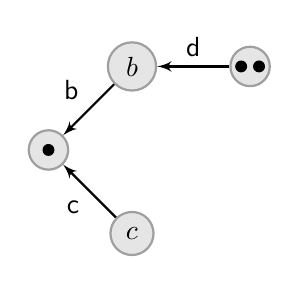
\begin{tikzpicture}[node distance=1.5cm,>=latex',bend angle=45,auto]
    \tikzstyle{place}=[circle,thick,draw=gray!75,fill=gray!20,minimum size=5mm]
    \begin{scope}[xshift=0cm,yshift=0cm]
        \node[place,tokens=1] (a) {};
        \draw[below] (a.south) node {};
        \node[above right of=a,place] (b) {$b$};
        \draw[below] (b.south) node {};
        \node[below right of=a,place] (c) {$c$};
        \draw[below] (c.south) node {};
        \node[right of=b,place,tokens=2] (d) {};
        \draw[below] (d.south) node {};
        \draw[<-,thick] (b) -- node[above] {$\d$} (d);
        \draw[<-,thick] (a) -- node[above left] {$\b$} (b);
        \draw[<-,thick] (a) -- node[below left] {$\c$} (c);
    \end{scope}
\end{tikzpicture}

\end{document}

